\documentclass[1p]{elsarticle_modified}
%\bibliographystyle{elsarticle-num}

%\usepackage[colorlinks]{hyperref}
%\usepackage{abbrmath_seonhwa} %\Abb, \Ascr, \Acal ,\Abf, \Afrak
\usepackage{amsfonts}
\usepackage{amssymb}
\usepackage{amsmath}
\usepackage{amsthm}
\usepackage{scalefnt}
\usepackage{amsbsy}
\usepackage{kotex}
\usepackage{caption}
\usepackage{subfig}
\usepackage{color}
\usepackage{graphicx}
\usepackage{xcolor} %% white, black, red, green, blue, cyan, magenta, yellow
\usepackage{float}
\usepackage{setspace}
\usepackage{hyperref}

\usepackage{tikz}
\usetikzlibrary{arrows}

\usepackage{multirow}
\usepackage{array} % fixed length table
\usepackage{hhline}

%%%%%%%%%%%%%%%%%%%%%
\makeatletter
\renewcommand*\env@matrix[1][\arraystretch]{%
	\edef\arraystretch{#1}%
	\hskip -\arraycolsep
	\let\@ifnextchar\new@ifnextchar
	\array{*\c@MaxMatrixCols c}}
\makeatother %https://tex.stackexchange.com/questions/14071/how-can-i-increase-the-line-spacing-in-a-matrix
%%%%%%%%%%%%%%%

\usepackage[normalem]{ulem}

\newcommand{\msout}[1]{\ifmmode\text{\sout{\ensuremath{#1}}}\else\sout{#1}\fi}
%SOURCE: \msout is \stkout macro in https://tex.stackexchange.com/questions/20609/strikeout-in-math-mode

\newcommand{\cancel}[1]{
	\ifmmode
	{\color{red}\msout{#1}}
	\else
	{\color{red}\sout{#1}}
	\fi
}

\newcommand{\add}[1]{
	{\color{blue}\uwave{#1}}
}

\newcommand{\replace}[2]{
	\ifmmode
	{\color{red}\msout{#1}}{\color{blue}\uwave{#2}}
	\else
	{\color{red}\sout{#1}}{\color{blue}\uwave{#2}}
	\fi
}

\newcommand{\Sol}{\mathcal{S}} %segment
\newcommand{\D}{D} %diagram
\newcommand{\A}{\mathcal{A}} %arc


%%%%%%%%%%%%%%%%%%%%%%%%%%%%%5 test

\def\sl{\operatorname{\textup{SL}}(2,\Cbb)}
\def\psl{\operatorname{\textup{PSL}}(2,\Cbb)}
\def\quan{\mkern 1mu \triangleright \mkern 1mu}

\theoremstyle{definition}
\newtheorem{thm}{Theorem}[section]
\newtheorem{prop}[thm]{Proposition}
\newtheorem{lem}[thm]{Lemma}
\newtheorem{ques}[thm]{Question}
\newtheorem{cor}[thm]{Corollary}
\newtheorem{defn}[thm]{Definition}
\newtheorem{exam}[thm]{Example}
\newtheorem{rmk}[thm]{Remark}
\newtheorem{alg}[thm]{Algorithm}

\newcommand{\I}{\sqrt{-1}}
\begin{document}

%\begin{frontmatter}
%
%\title{Boundary parabolic representations of knots up to 8 crossings}
%
%%% Group authors per affiliation:
%\author{Yunhi Cho} 
%\address{Department of Mathematics, University of Seoul, Seoul, Korea}
%\ead{yhcho@uos.ac.kr}
%
%
%\author{Seonhwa Kim} %\fnref{s_kim}}
%\address{Center for Geometry and Physics, Institute for Basic Science, Pohang, 37673, Korea}
%\ead{ryeona17@ibs.re.kr}
%
%\author{Hyuk Kim}
%\address{Department of Mathematical Sciences, Seoul National University, Seoul 08826, Korea}
%\ead{hyukkim@snu.ac.kr}
%
%\author{Seokbeom Yoon}
%\address{Department of Mathematical Sciences, Seoul National University, Seoul, 08826,  Korea}
%\ead{sbyoon15@snu.ac.kr}
%
%\begin{abstract}
%We find all boundary parabolic representation of knots up to 8 crossings.
%
%\end{abstract}
%\begin{keyword}
%    \MSC[2010] 57M25 
%\end{keyword}
%
%\end{frontmatter}

%\linenumbers
%\tableofcontents
%
\newcommand\colored[1]{\textcolor{white}{\rule[-0.35ex]{0.8em}{1.4ex}}\kern-0.8em\color{red} #1}%
%\newcommand\colored[1]{\textcolor{white}{ #1}\kern-2.17ex	\textcolor{white}{ #1}\kern-1.81ex	\textcolor{white}{ #1}\kern-2.15ex\color{red}#1	}

{\Large $\underline{12a_{0572}~(K12a_{0572})}$}

\setlength{\tabcolsep}{10pt}
\renewcommand{\arraystretch}{1.6}
\vspace{1cm}\begin{tabular}{m{100pt}>{\centering\arraybackslash}m{274pt}}
\multirow{5}{120pt}{
	\centering
	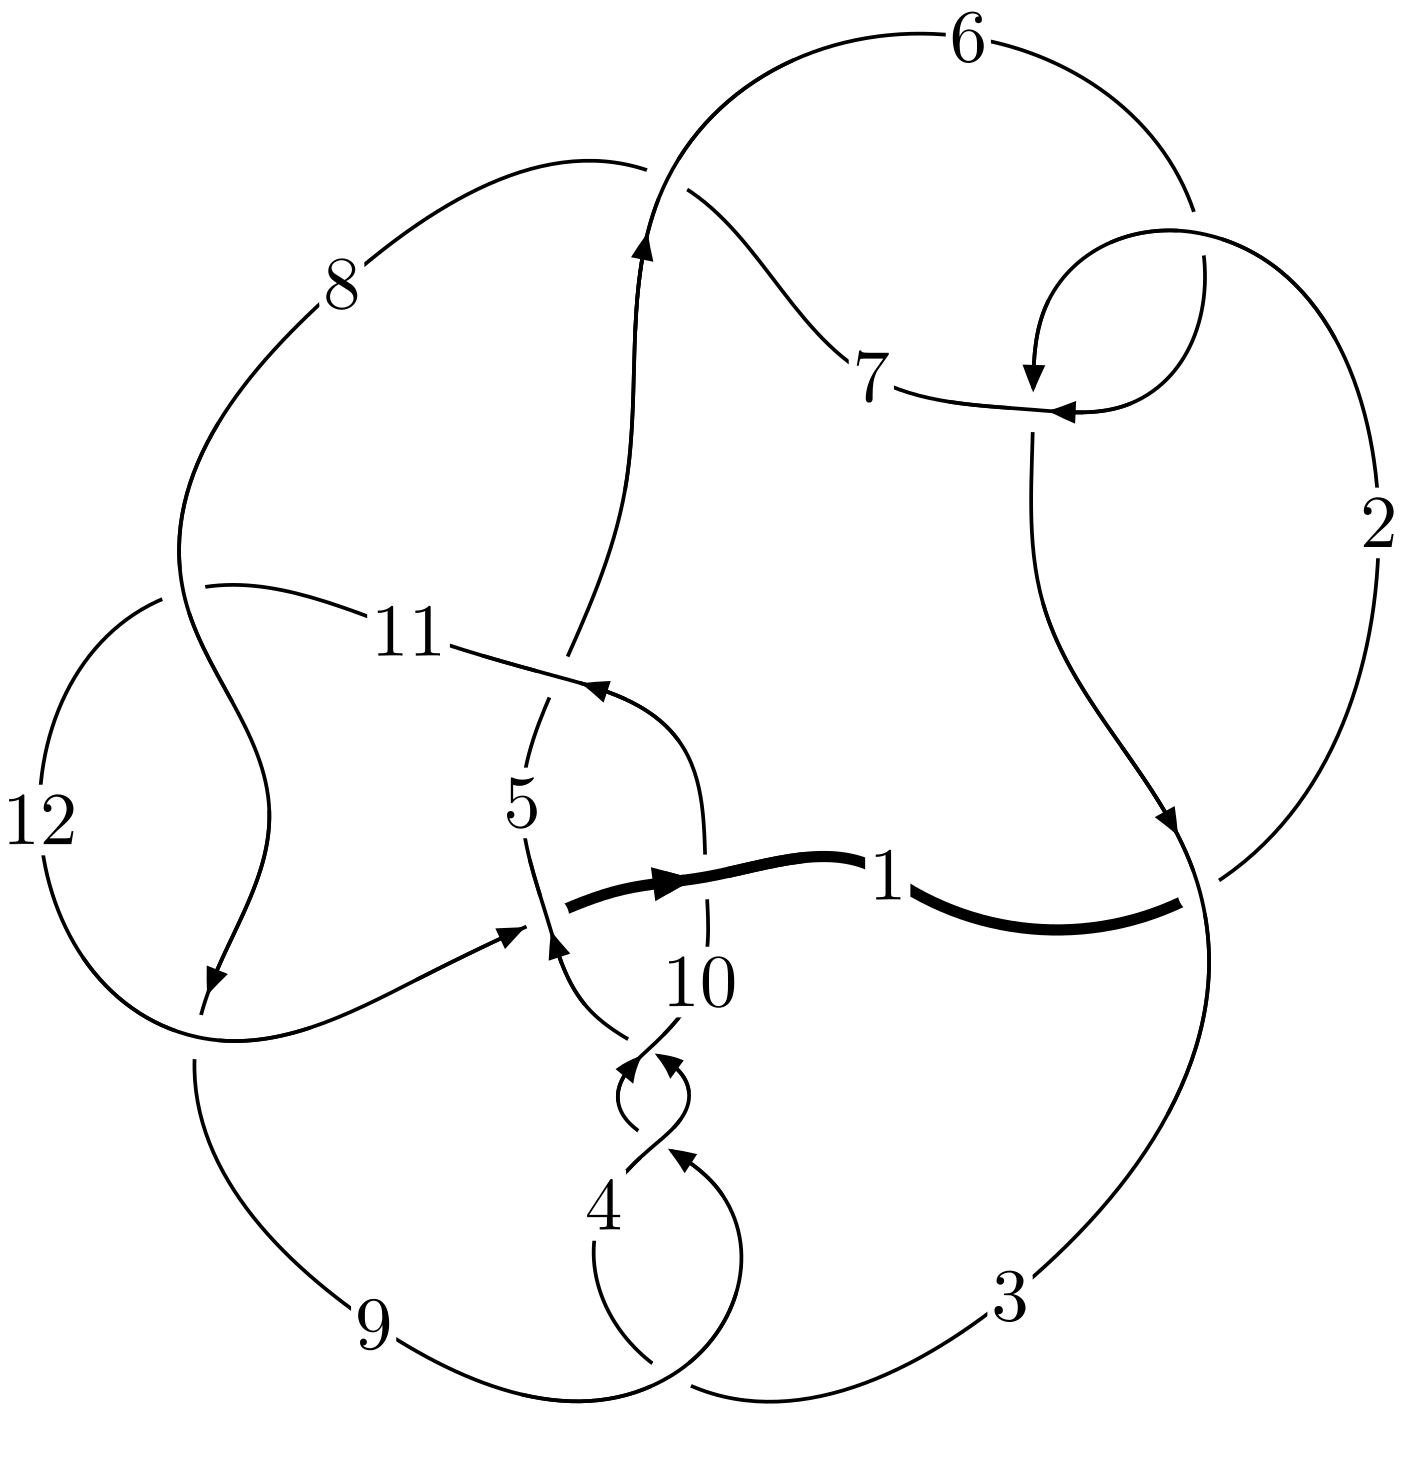
\includegraphics[width=112pt]{../../../GIT/diagram.site/Diagrams/png/1373_12a_0572.png}\\
\ \ \ A knot diagram\footnotemark}&
\allowdisplaybreaks
\textbf{Linearized knot diagam} \\
\cline{2-2}
 &
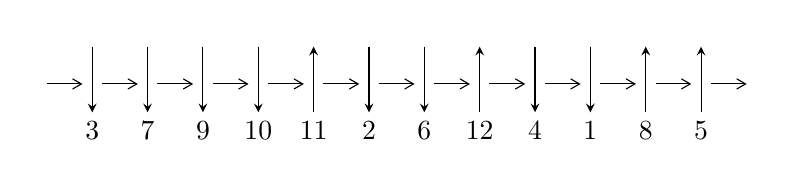
\begin{tikzpicture}[x=20pt, y=17pt]
	% nodes
	\node (C0) at (0, 0) {};
	\node (C1) at (1, 0) {};
	\node (C1U) at (1, +1) {};
	\node (C1D) at (1, -1) {3};

	\node (C2) at (2, 0) {};
	\node (C2U) at (2, +1) {};
	\node (C2D) at (2, -1) {7};

	\node (C3) at (3, 0) {};
	\node (C3U) at (3, +1) {};
	\node (C3D) at (3, -1) {9};

	\node (C4) at (4, 0) {};
	\node (C4U) at (4, +1) {};
	\node (C4D) at (4, -1) {10};

	\node (C5) at (5, 0) {};
	\node (C5U) at (5, +1) {};
	\node (C5D) at (5, -1) {11};

	\node (C6) at (6, 0) {};
	\node (C6U) at (6, +1) {};
	\node (C6D) at (6, -1) {2};

	\node (C7) at (7, 0) {};
	\node (C7U) at (7, +1) {};
	\node (C7D) at (7, -1) {6};

	\node (C8) at (8, 0) {};
	\node (C8U) at (8, +1) {};
	\node (C8D) at (8, -1) {12};

	\node (C9) at (9, 0) {};
	\node (C9U) at (9, +1) {};
	\node (C9D) at (9, -1) {4};

	\node (C10) at (10, 0) {};
	\node (C10U) at (10, +1) {};
	\node (C10D) at (10, -1) {1};

	\node (C11) at (11, 0) {};
	\node (C11U) at (11, +1) {};
	\node (C11D) at (11, -1) {8};

	\node (C12) at (12, 0) {};
	\node (C12U) at (12, +1) {};
	\node (C12D) at (12, -1) {5};
	\node (C13) at (13, 0) {};

	% arrows
	\draw[->,>={angle 60}]
	(C0) edge (C1) (C1) edge (C2) (C2) edge (C3) (C3) edge (C4) (C4) edge (C5) (C5) edge (C6) (C6) edge (C7) (C7) edge (C8) (C8) edge (C9) (C9) edge (C10) (C10) edge (C11) (C11) edge (C12) (C12) edge (C13) ;	\draw[->,>=stealth]
	(C1U) edge (C1D) (C2U) edge (C2D) (C3U) edge (C3D) (C4U) edge (C4D) (C5D) edge (C5U) (C6U) edge (C6D) (C7U) edge (C7D) (C8D) edge (C8U) (C9U) edge (C9D) (C10U) edge (C10D) (C11D) edge (C11U) (C12D) edge (C12U) ;
	\end{tikzpicture} \\
\hhline{~~} \\& 
\textbf{Solving Sequence} \\ \cline{2-2} 
 &
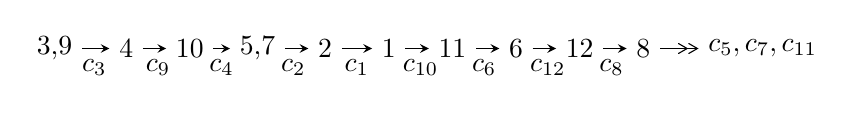
\begin{tikzpicture}[x=23pt, y=7pt]
	% node
	\node (A0) at (-1/8, 0) {3,9};
	\node (A1) at (1, 0) {4};
	\node (A2) at (2, 0) {10};
	\node (A3) at (49/16, 0) {5,7};
	\node (A4) at (33/8, 0) {2};
	\node (A5) at (41/8, 0) {1};
	\node (A6) at (49/8, 0) {11};
	\node (A7) at (57/8, 0) {6};
	\node (A8) at (65/8, 0) {12};
	\node (A9) at (73/8, 0) {8};
	\node (C1) at (1/2, -1) {$c_{3}$};
	\node (C2) at (3/2, -1) {$c_{9}$};
	\node (C3) at (5/2, -1) {$c_{4}$};
	\node (C4) at (29/8, -1) {$c_{2}$};
	\node (C5) at (37/8, -1) {$c_{1}$};
	\node (C6) at (45/8, -1) {$c_{10}$};
	\node (C7) at (53/8, -1) {$c_{6}$};
	\node (C8) at (61/8, -1) {$c_{12}$};
	\node (C9) at (69/8, -1) {$c_{8}$};
	\node (A10) at (11, 0) {$c_{5},c_{7},c_{11}$};

	% edge
	\draw[->,>=stealth]	
	(A0) edge (A1) (A1) edge (A2) (A2) edge (A3) (A3) edge (A4) (A4) edge (A5) (A5) edge (A6) (A6) edge (A7) (A7) edge (A8) (A8) edge (A9) ;
	\draw[->>,>={angle 60}]	
	(A9) edge (A10);
\end{tikzpicture} \\ 

\end{tabular} \\

\footnotetext{
The image of knot diagram is generated by the software ``\textbf{Draw programme}" developed by Andrew Bartholomew(\url{http://www.layer8.co.uk/maths/draw/index.htm\#Running-draw}), where we modified some parts for our purpose(\url{https://github.com/CATsTAILs/LinksPainter}).
}\phantom \\ \newline 
\centering \textbf{Ideals for irreducible components\footnotemark of $X_{\text{par}}$} 
 
\begin{align*}
I^u_{1}&=\langle 
2.15099\times10^{151} u^{95}+6.01892\times10^{150} u^{94}+\cdots+4.57032\times10^{151} b-4.06184\times10^{152},\\
\phantom{I^u_{1}}&\phantom{= \langle  }9.03162\times10^{152} u^{95}+5.47605\times10^{150} u^{94}+\cdots+1.32539\times10^{153} a-1.93189\times10^{154},\\
\phantom{I^u_{1}}&\phantom{= \langle  }u^{96}+u^{95}+\cdots-254 u-29\rangle \\
I^u_{2}&=\langle 
6 u^{22}-63 u^{20}+\cdots+b-7,\;-5 u^{22}+8 u^{21}+\cdots+a+1,\;u^{24}-12 u^{22}+\cdots-2 u+1\rangle \\
I^u_{3}&=\langle 
- u^{10}+2 u^8+u^6- u^5-2 u^4+u^3- u^2+b+u-1,\;u^{13}-2 u^{11}- u^9+2 u^7+2 u^5+a- u,\\
\phantom{I^u_{3}}&\phantom{= \langle  }u^{15}-3 u^{13}+u^{10}+5 u^9-2 u^8- u^6- u^5+2 u^4-3 u^3+u^2-2 u+1\rangle \\
\\
\end{align*}
\raggedright * 3 irreducible components of $\dim_{\mathbb{C}}=0$, with total 135 representations.\\
\footnotetext{All coefficients of polynomials are rational numbers. But the coefficients are sometimes approximated in decimal forms when there is not enough margin.}
\newpage
\renewcommand{\arraystretch}{1}
\centering \section*{I. $I^u_{1}= \langle 2.15\times10^{151} u^{95}+6.02\times10^{150} u^{94}+\cdots+4.57\times10^{151} b-4.06\times10^{152},\;9.03\times10^{152} u^{95}+5.48\times10^{150} u^{94}+\cdots+1.33\times10^{153} a-1.93\times10^{154},\;u^{96}+u^{95}+\cdots-254 u-29 \rangle$}
\flushleft \textbf{(i) Arc colorings}\\
\begin{tabular}{m{7pt} m{180pt} m{7pt} m{180pt} }
\flushright $a_{3}=$&$\begin{pmatrix}1\\0\end{pmatrix}$ \\
\flushright $a_{9}=$&$\begin{pmatrix}0\\u\end{pmatrix}$ \\
\flushright $a_{4}=$&$\begin{pmatrix}1\\u^2\end{pmatrix}$ \\
\flushright $a_{10}=$&$\begin{pmatrix}- u\\- u^3+u\end{pmatrix}$ \\
\flushright $a_{5}=$&$\begin{pmatrix}- u^2+1\\- u^4+2 u^2\end{pmatrix}$ \\
\flushright $a_{7}=$&$\begin{pmatrix}-0.681430 u^{95}-0.00413165 u^{94}+\cdots+99.7765 u+14.5760\\-0.470644 u^{95}-0.131696 u^{94}+\cdots+59.7808 u+8.88743\end{pmatrix}$ \\
\flushright $a_{2}=$&$\begin{pmatrix}-1.65395 u^{95}+0.429407 u^{94}+\cdots+386.874 u+50.3558\\1.07387 u^{95}-0.384746 u^{94}+\cdots-206.119 u-26.2557\end{pmatrix}$ \\
\flushright $a_{1}=$&$\begin{pmatrix}-0.580085 u^{95}+0.0446613 u^{94}+\cdots+180.755 u+24.1002\\1.07387 u^{95}-0.384746 u^{94}+\cdots-206.119 u-26.2557\end{pmatrix}$ \\
\flushright $a_{11}=$&$\begin{pmatrix}-0.454721 u^{95}+0.151308 u^{94}+\cdots+126.982 u+19.7118\\-0.351241 u^{95}+0.320756 u^{94}+\cdots+93.4406 u+11.4080\end{pmatrix}$ \\
\flushright $a_{6}=$&$\begin{pmatrix}0.308554 u^{95}+0.0963542 u^{94}+\cdots+42.1533 u+2.60418\\-1.17149 u^{95}-0.204140 u^{94}+\cdots+153.030 u+21.0519\end{pmatrix}$ \\
\flushright $a_{12}=$&$\begin{pmatrix}-0.888517 u^{95}+0.0913258 u^{94}+\cdots+249.933 u+33.1094\\1.29641 u^{95}-0.491042 u^{94}+\cdots-246.556 u-30.8209\end{pmatrix}$ \\
\flushright $a_{8}=$&$\begin{pmatrix}0.922646 u^{95}-0.276868 u^{94}+\cdots-54.9860 u-3.07145\\0.00159182 u^{95}-0.299162 u^{94}+\cdots-85.6322 u-10.7903\end{pmatrix}$\\&\end{tabular}
\flushleft \textbf{(ii) Obstruction class $= -1$}\\~\\
\flushleft \textbf{(iii) Cusp Shapes $= -4.21551 u^{95}+2.24153 u^{94}+\cdots+978.183 u+121.935$}\\~\\
\newpage\renewcommand{\arraystretch}{1}
\flushleft \textbf{(iv) u-Polynomials at the component}\newline \\
\begin{tabular}{m{50pt}|m{274pt}}
Crossings & \hspace{64pt}u-Polynomials at each crossing \\
\hline $$\begin{aligned}c_{1},c_{7}\end{aligned}$$&$\begin{aligned}
&u^{96}+30 u^{95}+\cdots+140 u+16
\end{aligned}$\\
\hline $$\begin{aligned}c_{2},c_{6}\end{aligned}$$&$\begin{aligned}
&u^{96}+4 u^{95}+\cdots-14 u+4
\end{aligned}$\\
\hline $$\begin{aligned}c_{3},c_{4},c_{9}\end{aligned}$$&$\begin{aligned}
&u^{96}- u^{95}+\cdots+254 u-29
\end{aligned}$\\
\hline $$\begin{aligned}c_{5}\end{aligned}$$&$\begin{aligned}
&u^{96}+u^{95}+\cdots-128495 u-83681
\end{aligned}$\\
\hline $$\begin{aligned}c_{8},c_{11}\end{aligned}$$&$\begin{aligned}
&u^{96}-5 u^{95}+\cdots+50782 u+9913
\end{aligned}$\\
\hline $$\begin{aligned}c_{10}\end{aligned}$$&$\begin{aligned}
&u^{96}-11 u^{95}+\cdots+3726 u-783
\end{aligned}$\\
\hline $$\begin{aligned}c_{12}\end{aligned}$$&$\begin{aligned}
&u^{96}-4 u^{95}+\cdots+994 u-121
\end{aligned}$\\
\hline
\end{tabular}\\~\\
\newpage\renewcommand{\arraystretch}{1}
\flushleft \textbf{(v) Riley Polynomials at the component}\newline \\
\begin{tabular}{m{50pt}|m{274pt}}
Crossings & \hspace{64pt}Riley Polynomials at each crossing \\
\hline $$\begin{aligned}c_{1},c_{7}\end{aligned}$$&$\begin{aligned}
&y^{96}+78 y^{95}+\cdots-64624 y+256
\end{aligned}$\\
\hline $$\begin{aligned}c_{2},c_{6}\end{aligned}$$&$\begin{aligned}
&y^{96}-30 y^{95}+\cdots-140 y+16
\end{aligned}$\\
\hline $$\begin{aligned}c_{3},c_{4},c_{9}\end{aligned}$$&$\begin{aligned}
&y^{96}-99 y^{95}+\cdots+618 y+841
\end{aligned}$\\
\hline $$\begin{aligned}c_{5}\end{aligned}$$&$\begin{aligned}
&y^{96}-43 y^{95}+\cdots-297276786777 y+7002509761
\end{aligned}$\\
\hline $$\begin{aligned}c_{8},c_{11}\end{aligned}$$&$\begin{aligned}
&y^{96}-67 y^{95}+\cdots-2596436838 y+98267569
\end{aligned}$\\
\hline $$\begin{aligned}c_{10}\end{aligned}$$&$\begin{aligned}
&y^{96}+5 y^{95}+\cdots-16105230 y+613089
\end{aligned}$\\
\hline $$\begin{aligned}c_{12}\end{aligned}$$&$\begin{aligned}
&y^{96}+14 y^{95}+\cdots+401770 y+14641
\end{aligned}$\\
\hline
\end{tabular}\\~\\
\newpage\flushleft \textbf{(vi) Complex Volumes and Cusp Shapes}
$$\begin{array}{c|c|c}  
\text{Solutions to }I^u_{1}& \I (\text{vol} + \sqrt{-1}CS) & \text{Cusp shape}\\
 \hline 
\begin{aligned}
u &= \phantom{-}0.385743 + 0.920287 I \\
a &= -0.26339 - 2.22738 I \\
b &= \phantom{-}1.018312 + 0.780274 I\end{aligned}
 & \phantom{-}7.3635 - 13.1198 I & \phantom{-0.000000 } 0 \\ \hline\begin{aligned}
u &= \phantom{-}0.385743 - 0.920287 I \\
a &= -0.26339 + 2.22738 I \\
b &= \phantom{-}1.018312 - 0.780274 I\end{aligned}
 & \phantom{-}7.3635 + 13.1198 I & \phantom{-0.000000 } 0 \\ \hline\begin{aligned}
u &= \phantom{-}0.663242 + 0.767263 I \\
a &= -0.093897 - 0.238168 I \\
b &= \phantom{-}0.979786 - 0.185667 I\end{aligned}
 & -0.04698 + 2.47024 I & \phantom{-0.000000 } 0 \\ \hline\begin{aligned}
u &= \phantom{-}0.663242 - 0.767263 I \\
a &= -0.093897 + 0.238168 I \\
b &= \phantom{-}0.979786 + 0.185667 I\end{aligned}
 & -0.04698 - 2.47024 I & \phantom{-0.000000 } 0 \\ \hline\begin{aligned}
u &= -0.354084 + 0.893077 I \\
a &= -1.21039 - 1.32767 I \\
b &= \phantom{-}0.746214 + 0.886048 I\end{aligned}
 & \phantom{-}8.21230 + 6.94201 I & \phantom{-0.000000 } 0 \\ \hline\begin{aligned}
u &= -0.354084 - 0.893077 I \\
a &= -1.21039 + 1.32767 I \\
b &= \phantom{-}0.746214 - 0.886048 I\end{aligned}
 & \phantom{-}8.21230 - 6.94201 I & \phantom{-0.000000 } 0 \\ \hline\begin{aligned}
u &= \phantom{-}0.135681 + 0.893536 I \\
a &= \phantom{-}0.68169 + 1.79557 I \\
b &= -0.865194 - 0.590369 I\end{aligned}
 & \phantom{-}1.68985 - 2.34367 I & \phantom{-0.000000 } 0 \\ \hline\begin{aligned}
u &= \phantom{-}0.135681 - 0.893536 I \\
a &= \phantom{-}0.68169 - 1.79557 I \\
b &= -0.865194 + 0.590369 I\end{aligned}
 & \phantom{-}1.68985 + 2.34367 I & \phantom{-0.000000 } 0 \\ \hline\begin{aligned}
u &= \phantom{-}0.471081 + 0.760470 I \\
a &= -0.013155 + 1.084280 I \\
b &= -1.075187 - 0.289861 I\end{aligned}
 & \phantom{-}0.38982 - 7.56346 I & \phantom{-0.000000 } 0 \\ \hline\begin{aligned}
u &= \phantom{-}0.471081 - 0.760470 I \\
a &= -0.013155 - 1.084280 I \\
b &= -1.075187 + 0.289861 I\end{aligned}
 & \phantom{-}0.38982 + 7.56346 I & \phantom{-0.000000 } 0\\
 \hline 
 \end{array}$$\newpage$$\begin{array}{c|c|c}  
\text{Solutions to }I^u_{1}& \I (\text{vol} + \sqrt{-1}CS) & \text{Cusp shape}\\
 \hline 
\begin{aligned}
u &= -0.935682 + 0.714738 I \\
a &= \phantom{-}0.04944 - 1.74878 I \\
b &= -0.760190 + 0.824141 I\end{aligned}
 & \phantom{-}6.56134 - 1.43456 I & \phantom{-0.000000 } 0 \\ \hline\begin{aligned}
u &= -0.935682 - 0.714738 I \\
a &= \phantom{-}0.04944 + 1.74878 I \\
b &= -0.760190 - 0.824141 I\end{aligned}
 & \phantom{-}6.56134 + 1.43456 I & \phantom{-0.000000 } 0 \\ \hline\begin{aligned}
u &= -0.468471 + 0.659668 I \\
a &= \phantom{-}0.40771 + 2.35136 I \\
b &= \phantom{-}0.943827 - 0.759298 I\end{aligned}
 & \phantom{-}2.98434 + 7.28558 I & \phantom{-0.000000 } 0 \\ \hline\begin{aligned}
u &= -0.468471 - 0.659668 I \\
a &= \phantom{-}0.40771 - 2.35136 I \\
b &= \phantom{-}0.943827 + 0.759298 I\end{aligned}
 & \phantom{-}2.98434 - 7.28558 I & \phantom{-0.000000 } 0 \\ \hline\begin{aligned}
u &= \phantom{-}0.924493 + 0.776710 I \\
a &= \phantom{-}0.657518 - 1.023712 I \\
b &= -0.986223 + 0.755241 I\end{aligned}
 & \phantom{-}5.86427 + 7.35566 I & \phantom{-0.000000 } 0 \\ \hline\begin{aligned}
u &= \phantom{-}0.924493 - 0.776710 I \\
a &= \phantom{-}0.657518 + 1.023712 I \\
b &= -0.986223 - 0.755241 I\end{aligned}
 & \phantom{-}5.86427 - 7.35566 I & \phantom{-0.000000 } 0 \\ \hline\begin{aligned}
u &= \phantom{-}0.412450 + 0.664332 I \\
a &= -1.38768 + 0.63963 I \\
b &= \phantom{-}0.809782 - 0.789448 I\end{aligned}
 & \phantom{-}3.39395 - 1.44923 I & \phantom{-0.000000 } 0 \\ \hline\begin{aligned}
u &= \phantom{-}0.412450 - 0.664332 I \\
a &= -1.38768 - 0.63963 I \\
b &= \phantom{-}0.809782 + 0.789448 I\end{aligned}
 & \phantom{-}3.39395 + 1.44923 I & \phantom{-0.000000 } 0 \\ \hline\begin{aligned}
u &= -0.334080 + 0.660105 I \\
a &= \phantom{-}0.066401 + 1.330555 I \\
b &= -0.025158 - 0.783113 I\end{aligned}
 & \phantom{-}3.89051 + 3.95952 I & \phantom{-}2.70271 - 5.67794 I \\ \hline\begin{aligned}
u &= -0.334080 - 0.660105 I \\
a &= \phantom{-}0.066401 - 1.330555 I \\
b &= -0.025158 + 0.783113 I\end{aligned}
 & \phantom{-}3.89051 - 3.95952 I & \phantom{-}2.70271 + 5.67794 I\\
 \hline 
 \end{array}$$\newpage$$\begin{array}{c|c|c}  
\text{Solutions to }I^u_{1}& \I (\text{vol} + \sqrt{-1}CS) & \text{Cusp shape}\\
 \hline 
\begin{aligned}
u &= -1.265687 + 0.164608 I \\
a &= -0.305186 + 0.194936 I \\
b &= \phantom{-}0.618688 + 0.905355 I\end{aligned}
 & \phantom{-}4.18322 + 1.97592 I & \phantom{-0.000000 } 0 \\ \hline\begin{aligned}
u &= -1.265687 - 0.164608 I \\
a &= -0.305186 - 0.194936 I \\
b &= \phantom{-}0.618688 - 0.905355 I\end{aligned}
 & \phantom{-}4.18322 - 1.97592 I & \phantom{-0.000000 } 0 \\ \hline\begin{aligned}
u &= -1.270790 + 0.120676 I \\
a &= -0.100143 - 0.807864 I \\
b &= \phantom{-}0.999396 + 0.869415 I\end{aligned}
 & \phantom{-}3.52668 - 3.66382 I & \phantom{-0.000000 } 0 \\ \hline\begin{aligned}
u &= -1.270790 - 0.120676 I \\
a &= -0.100143 + 0.807864 I \\
b &= \phantom{-}0.999396 - 0.869415 I\end{aligned}
 & \phantom{-}3.52668 + 3.66382 I & \phantom{-0.000000 } 0 \\ \hline\begin{aligned}
u &= -0.609687 + 0.366846 I \\
a &= \phantom{-}1.58577 + 0.87904 I \\
b &= \phantom{-}0.007089 - 0.413591 I\end{aligned}
 & \phantom{-}2.89097 - 0.23399 I & \phantom{-}2.30056 - 1.02334 I \\ \hline\begin{aligned}
u &= -0.609687 - 0.366846 I \\
a &= \phantom{-}1.58577 - 0.87904 I \\
b &= \phantom{-}0.007089 + 0.413591 I\end{aligned}
 & \phantom{-}2.89097 + 0.23399 I & \phantom{-}2.30056 + 1.02334 I \\ \hline\begin{aligned}
u &= \phantom{-}1.29120\phantom{ +0.000000I} \\
a &= -1.61139\phantom{ +0.000000I} \\
b &= -1.30175\phantom{ +0.000000I}\end{aligned}
 & -2.81463\phantom{ +0.000000I} & \phantom{-0.000000 } 0 \\ \hline\begin{aligned}
u &= \phantom{-}1.295518 + 0.112046 I \\
a &= \phantom{-}1.12403 - 1.32519 I \\
b &= -0.867065 + 0.855609 I\end{aligned}
 & \phantom{-}3.57768 - 1.08471 I & \phantom{-0.000000 } 0 \\ \hline\begin{aligned}
u &= \phantom{-}1.295518 - 0.112046 I \\
a &= \phantom{-}1.12403 + 1.32519 I \\
b &= -0.867065 - 0.855609 I\end{aligned}
 & \phantom{-}3.57768 + 1.08471 I & \phantom{-0.000000 } 0 \\ \hline\begin{aligned}
u &= -1.294278 + 0.128891 I \\
a &= \phantom{-}0.27458 - 2.17732 I \\
b &= -0.938756 + 0.826704 I\end{aligned}
 & \phantom{-}3.35105 + 7.33768 I & \phantom{-0.000000 } 0\\
 \hline 
 \end{array}$$\newpage$$\begin{array}{c|c|c}  
\text{Solutions to }I^u_{1}& \I (\text{vol} + \sqrt{-1}CS) & \text{Cusp shape}\\
 \hline 
\begin{aligned}
u &= -1.294278 - 0.128891 I \\
a &= \phantom{-}0.27458 + 2.17732 I \\
b &= -0.938756 - 0.826704 I\end{aligned}
 & \phantom{-}3.35105 - 7.33768 I & \phantom{-0.000000 } 0 \\ \hline\begin{aligned}
u &= \phantom{-}1.294428 + 0.156264 I \\
a &= \phantom{-}0.096525 - 1.097000 I \\
b &= \phantom{-}0.834667 + 0.951948 I\end{aligned}
 & \phantom{-}4.05073 - 2.99694 I & \phantom{-0.000000 } 0 \\ \hline\begin{aligned}
u &= \phantom{-}1.294428 - 0.156264 I \\
a &= \phantom{-}0.096525 + 1.097000 I \\
b &= \phantom{-}0.834667 - 0.951948 I\end{aligned}
 & \phantom{-}4.05073 + 2.99694 I & \phantom{-0.000000 } 0 \\ \hline\begin{aligned}
u &= \phantom{-}1.331300 + 0.160981 I \\
a &= \phantom{-}1.30482 - 1.22682 I \\
b &= \phantom{-}1.084050 + 0.751190 I\end{aligned}
 & \phantom{-}2.77719 - 8.10147 I & \phantom{-0.000000 } 0 \\ \hline\begin{aligned}
u &= \phantom{-}1.331300 - 0.160981 I \\
a &= \phantom{-}1.30482 + 1.22682 I \\
b &= \phantom{-}1.084050 - 0.751190 I\end{aligned}
 & \phantom{-}2.77719 + 8.10147 I & \phantom{-0.000000 } 0 \\ \hline\begin{aligned}
u &= -0.460716 + 0.424248 I \\
a &= -1.31371 - 0.93039 I \\
b &= -0.910181 + 0.209562 I\end{aligned}
 & -2.75688 + 3.28834 I & -10.53288 - 7.33652 I \\ \hline\begin{aligned}
u &= -0.460716 - 0.424248 I \\
a &= -1.31371 + 0.93039 I \\
b &= -0.910181 - 0.209562 I\end{aligned}
 & -2.75688 - 3.28834 I & -10.53288 + 7.33652 I \\ \hline\begin{aligned}
u &= -1.352914 + 0.252649 I \\
a &= -0.120568 + 0.331321 I \\
b &=                  -6
-0.394137 - 6. 10   I\end{aligned}
 & -4.97451 + 3.66414 I & \phantom{-0.000000 } 0 \\ \hline\begin{aligned}
u &= -1.352914 - 0.252649 I \\
a &= -0.120568 - 0.331321 I \\
b &=                  -6
-0.394137 + 6. 10   I\end{aligned}
 & -4.97451 - 3.66414 I & \phantom{-0.000000 } 0 \\ \hline\begin{aligned}
u &= -1.368542 + 0.152756 I \\
a &= -0.0128781 - 0.1160252 I \\
b &= -0.309216 + 0.563548 I\end{aligned}
 & -5.22850 + 3.47859 I & \phantom{-0.000000 } 0\\
 \hline 
 \end{array}$$\newpage$$\begin{array}{c|c|c}  
\text{Solutions to }I^u_{1}& \I (\text{vol} + \sqrt{-1}CS) & \text{Cusp shape}\\
 \hline 
\begin{aligned}
u &= -1.368542 - 0.152756 I \\
a &= -0.0128781 + 0.1160252 I \\
b &= -0.309216 - 0.563548 I\end{aligned}
 & -5.22850 - 3.47859 I & \phantom{-0.000000 } 0 \\ \hline\begin{aligned}
u &= \phantom{-}0.193262 + 0.570422 I \\
a &= \phantom{-}1.32752 + 1.93198 I \\
b &= -0.784388 - 0.291616 I\end{aligned}
 & \phantom{-}1.13940 - 2.20728 I & -0.01228 + 7.32813 I \\ \hline\begin{aligned}
u &= \phantom{-}0.193262 - 0.570422 I \\
a &= \phantom{-}1.32752 - 1.93198 I \\
b &= -0.784388 + 0.291616 I\end{aligned}
 & \phantom{-}1.13940 + 2.20728 I & -0.01228 - 7.32813 I \\ \hline\begin{aligned}
u &= \phantom{-}1.381065 + 0.233970 I \\
a &= -0.576924 + 0.538644 I \\
b &= \phantom{-}0.559104 - 0.738166 I\end{aligned}
 & -2.50654 - 1.42565 I & \phantom{-0.000000 } 0 \\ \hline\begin{aligned}
u &= \phantom{-}1.381065 - 0.233970 I \\
a &= -0.576924 - 0.538644 I \\
b &= \phantom{-}0.559104 + 0.738166 I\end{aligned}
 & -2.50654 + 1.42565 I & \phantom{-0.000000 } 0 \\ \hline\begin{aligned}
u &= -1.395635 + 0.184655 I \\
a &= \phantom{-}0.127249 + 1.274073 I \\
b &= \phantom{-}0.723765 - 0.418716 I\end{aligned}
 & -3.90744 + 4.87063 I & \phantom{-0.000000 } 0 \\ \hline\begin{aligned}
u &= -1.395635 - 0.184655 I \\
a &= \phantom{-}0.127249 - 1.274073 I \\
b &= \phantom{-}0.723765 + 0.418716 I\end{aligned}
 & -3.90744 - 4.87063 I & \phantom{-0.000000 } 0 \\ \hline\begin{aligned}
u &= \phantom{-}1.409053 + 0.067170 I \\
a &= -1.28444 - 0.74008 I \\
b &= -1.025047 + 0.466204 I\end{aligned}
 & -7.26522 + 0.62596 I & \phantom{-0.000000 } 0 \\ \hline\begin{aligned}
u &= \phantom{-}1.409053 - 0.067170 I \\
a &= -1.28444 + 0.74008 I \\
b &= -1.025047 - 0.466204 I\end{aligned}
 & -7.26522 - 0.62596 I & \phantom{-0.000000 } 0 \\ \hline\begin{aligned}
u &= \phantom{-}1.411271 + 0.017367 I \\
a &= -0.206449 + 0.766721 I \\
b &= \phantom{-}0.419657 - 0.629449 I\end{aligned}
 & -3.05064 - 0.91419 I & \phantom{-0.000000 } 0\\
 \hline 
 \end{array}$$\newpage$$\begin{array}{c|c|c}  
\text{Solutions to }I^u_{1}& \I (\text{vol} + \sqrt{-1}CS) & \text{Cusp shape}\\
 \hline 
\begin{aligned}
u &= \phantom{-}1.411271 - 0.017367 I \\
a &= -0.206449 - 0.766721 I \\
b &= \phantom{-}0.419657 + 0.629449 I\end{aligned}
 & -3.05064 + 0.91419 I & \phantom{-0.000000 } 0 \\ \hline\begin{aligned}
u &= -1.37464 + 0.44446 I \\
a &= -0.914447 - 0.786391 I \\
b &= \phantom{-}0.823552 + 0.765190 I\end{aligned}
 & -1.32824 + 2.49262 I & \phantom{-0.000000 } 0 \\ \hline\begin{aligned}
u &= -1.37464 - 0.44446 I \\
a &= -0.914447 + 0.786391 I \\
b &= \phantom{-}0.823552 - 0.765190 I\end{aligned}
 & -1.32824 - 2.49262 I & \phantom{-0.000000 } 0 \\ \hline\begin{aligned}
u &= -1.43821 + 0.17375 I \\
a &= -0.726188 + 0.114938 I \\
b &= -1.239035 - 0.341309 I\end{aligned}
 & -5.83118 + 2.77682 I & \phantom{-0.000000 } 0 \\ \hline\begin{aligned}
u &= -1.43821 - 0.17375 I \\
a &= -0.726188 - 0.114938 I \\
b &= -1.239035 + 0.341309 I\end{aligned}
 & -5.83118 - 2.77682 I & \phantom{-0.000000 } 0 \\ \hline\begin{aligned}
u &= \phantom{-}1.43393 + 0.24614 I \\
a &= -0.332589 + 0.576994 I \\
b &= -0.041356 - 0.913366 I\end{aligned}
 & -1.78579 - 7.25616 I & \phantom{-0.000000 } 0 \\ \hline\begin{aligned}
u &= \phantom{-}1.43393 - 0.24614 I \\
a &= -0.332589 - 0.576994 I \\
b &= -0.041356 + 0.913366 I\end{aligned}
 & -1.78579 + 7.25616 I & \phantom{-0.000000 } 0 \\ \hline\begin{aligned}
u &= \phantom{-}0.366601 + 0.388801 I \\
a &= -0.438408 + 0.713928 I \\
b &= \phantom{-}1.123777 - 0.216649 I\end{aligned}
 & -0.005958 - 0.537835 I & -2.51261 + 8.87589 I \\ \hline\begin{aligned}
u &= \phantom{-}0.366601 - 0.388801 I \\
a &= -0.438408 - 0.713928 I \\
b &= \phantom{-}1.123777 + 0.216649 I\end{aligned}
 & -0.005958 + 0.537835 I & -2.51261 - 8.87589 I \\ \hline\begin{aligned}
u &= -0.003669 + 0.531412 I \\
a &= \phantom{-}1.52604 - 1.37366 I \\
b &= -0.751294 + 0.914167 I\end{aligned}
 & \phantom{-}8.07625 + 0.55686 I & \phantom{-}5.81445 - 0.47058 I\\
 \hline 
 \end{array}$$\newpage$$\begin{array}{c|c|c}  
\text{Solutions to }I^u_{1}& \I (\text{vol} + \sqrt{-1}CS) & \text{Cusp shape}\\
 \hline 
\begin{aligned}
u &= -0.003669 - 0.531412 I \\
a &= \phantom{-}1.52604 + 1.37366 I \\
b &= -0.751294 - 0.914167 I\end{aligned}
 & \phantom{-}8.07625 - 0.55686 I & \phantom{-}5.81445 + 0.47058 I \\ \hline\begin{aligned}
u &= \phantom{-}1.46464 + 0.16428 I \\
a &= \phantom{-}1.64834 - 0.63689 I \\
b &= \phantom{-}1.016207 + 0.168687 I\end{aligned}
 & -8.98408 - 5.52910 I & \phantom{-0.000000 } 0 \\ \hline\begin{aligned}
u &= \phantom{-}1.46464 - 0.16428 I \\
a &= \phantom{-}1.64834 + 0.63689 I \\
b &= \phantom{-}1.016207 - 0.168687 I\end{aligned}
 & -8.98408 + 5.52910 I & \phantom{-0.000000 } 0 \\ \hline\begin{aligned}
u &= -1.45673 + 0.24384 I \\
a &= \phantom{-}0.662498 - 0.031069 I \\
b &= -0.756340 - 0.799979 I\end{aligned}
 & -2.60853 + 4.75653 I & \phantom{-0.000000 } 0 \\ \hline\begin{aligned}
u &= -1.45673 - 0.24384 I \\
a &= \phantom{-}0.662498 + 0.031069 I \\
b &= -0.756340 + 0.799979 I\end{aligned}
 & -2.60853 - 4.75653 I & \phantom{-0.000000 } 0 \\ \hline\begin{aligned}
u &= \phantom{-}0.242107 + 0.457342 I \\
a &= \phantom{-}0.346810 - 0.285860 I \\
b &= \phantom{-}0.029135 + 0.383175 I\end{aligned}
 & -0.180616 - 1.192610 I & -2.62815 + 5.38719 I \\ \hline\begin{aligned}
u &= \phantom{-}0.242107 - 0.457342 I \\
a &= \phantom{-}0.346810 + 0.285860 I \\
b &= \phantom{-}0.029135 - 0.383175 I\end{aligned}
 & -0.180616 + 1.192610 I & -2.62815 - 5.38719 I \\ \hline\begin{aligned}
u &= \phantom{-}1.41615 + 0.44982 I \\
a &= \phantom{-}0.37692 - 2.00054 I \\
b &= \phantom{-}0.926604 + 0.743757 I\end{aligned}
 & -1.64583 - 8.20716 I & \phantom{-0.000000 } 0 \\ \hline\begin{aligned}
u &= \phantom{-}1.41615 - 0.44982 I \\
a &= \phantom{-}0.37692 + 2.00054 I \\
b &= \phantom{-}0.926604 - 0.743757 I\end{aligned}
 & -1.64583 + 8.20716 I & \phantom{-0.000000 } 0 \\ \hline\begin{aligned}
u &= \phantom{-}1.47921 + 0.24044 I \\
a &= -1.18070 + 1.68873 I \\
b &= -0.980661 - 0.745233 I\end{aligned}
 & -3.29263 - 10.57900 I & \phantom{-0.000000 } 0\\
 \hline 
 \end{array}$$\newpage$$\begin{array}{c|c|c}  
\text{Solutions to }I^u_{1}& \I (\text{vol} + \sqrt{-1}CS) & \text{Cusp shape}\\
 \hline 
\begin{aligned}
u &= \phantom{-}1.47921 - 0.24044 I \\
a &= -1.18070 - 1.68873 I \\
b &= -0.980661 + 0.745233 I\end{aligned}
 & -3.29263 + 10.57900 I & \phantom{-0.000000 } 0 \\ \hline\begin{aligned}
u &= -1.47057 + 0.30015 I \\
a &= \phantom{-}0.63167 + 1.55832 I \\
b &= \phantom{-}1.032637 - 0.650837 I\end{aligned}
 & -3.88087 + 6.72339 I & \phantom{-0.000000 } 0 \\ \hline\begin{aligned}
u &= -1.47057 - 0.30015 I \\
a &= \phantom{-}0.63167 - 1.55832 I \\
b &= \phantom{-}1.032637 + 0.650837 I\end{aligned}
 & -3.88087 - 6.72339 I & \phantom{-0.000000 } 0 \\ \hline\begin{aligned}
u &= \phantom{-}1.46946 + 0.34201 I \\
a &= \phantom{-}0.833509 - 0.383063 I \\
b &= -0.723681 + 0.925712 I\end{aligned}
 & \phantom{-}2.37021 - 11.38420 I & \phantom{-0.000000 } 0 \\ \hline\begin{aligned}
u &= \phantom{-}1.46946 - 0.34201 I \\
a &= \phantom{-}0.833509 + 0.383063 I \\
b &= -0.723681 - 0.925712 I\end{aligned}
 & \phantom{-}2.37021 + 11.38420 I & \phantom{-0.000000 } 0 \\ \hline\begin{aligned}
u &= -0.037275 + 0.487405 I \\
a &= -3.41330 - 1.79895 I \\
b &= \phantom{-}0.925692 + 0.789261 I\end{aligned}
 & \phantom{-}7.25080 - 5.19343 I & \phantom{-}5.91357 + 5.53961 I \\ \hline\begin{aligned}
u &= -0.037275 - 0.487405 I \\
a &= -3.41330 + 1.79895 I \\
b &= \phantom{-}0.925692 - 0.789261 I\end{aligned}
 & \phantom{-}7.25080 + 5.19343 I & \phantom{-}5.91357 - 5.53961 I \\ \hline\begin{aligned}
u &= -0.067495 + 0.481964 I \\
a &= \phantom{-}0.27248 - 2.68237 I \\
b &= -1.028324 + 0.803320 I\end{aligned}
 & \phantom{-}7.21452 + 5.77752 I & \phantom{-}4.21585 - 6.14634 I \\ \hline\begin{aligned}
u &= -0.067495 - 0.481964 I \\
a &= \phantom{-}0.27248 + 2.68237 I \\
b &= -1.028324 - 0.803320 I\end{aligned}
 & \phantom{-}7.21452 - 5.77752 I & \phantom{-}4.21585 + 6.14634 I \\ \hline\begin{aligned}
u &= \phantom{-}1.47665 + 0.33190 I \\
a &= -1.11324 + 0.88392 I \\
b &= -0.860610 - 0.096616 I\end{aligned}
 & -6.57609 - 4.45340 I & \phantom{-0.000000 } 0\\
 \hline 
 \end{array}$$\newpage$$\begin{array}{c|c|c}  
\text{Solutions to }I^u_{1}& \I (\text{vol} + \sqrt{-1}CS) & \text{Cusp shape}\\
 \hline 
\begin{aligned}
u &= \phantom{-}1.47665 - 0.33190 I \\
a &= -1.11324 - 0.88392 I \\
b &= -0.860610 + 0.096616 I\end{aligned}
 & -6.57609 + 4.45340 I & \phantom{-0.000000 } 0 \\ \hline\begin{aligned}
u &= -1.49158 + 0.27180 I \\
a &= \phantom{-}0.963012 + 0.994212 I \\
b &= \phantom{-}1.166353 - 0.296461 I\end{aligned}
 & -5.94258 + 11.30370 I & \phantom{-0.000000 } 0 \\ \hline\begin{aligned}
u &= -1.49158 - 0.27180 I \\
a &= \phantom{-}0.963012 - 0.994212 I \\
b &= \phantom{-}1.166353 + 0.296461 I\end{aligned}
 & -5.94258 - 11.30370 I & \phantom{-0.000000 } 0 \\ \hline\begin{aligned}
u &= -1.52409 + 0.10872 I \\
a &= -1.003222 - 0.242752 I \\
b &= -1.076996 + 0.004087 I\end{aligned}
 & -7.97132 + 0.35100 I & \phantom{-0.000000 } 0 \\ \hline\begin{aligned}
u &= -1.52409 - 0.10872 I \\
a &= -1.003222 + 0.242752 I \\
b &= -1.076996 - 0.004087 I\end{aligned}
 & -7.97132 - 0.35100 I & \phantom{-0.000000 } 0 \\ \hline\begin{aligned}
u &= -1.48800 + 0.35029 I \\
a &= -0.76078 - 1.82949 I \\
b &= -1.046910 + 0.786981 I\end{aligned}
 & \phantom{-}1.3548 + 17.6950 I & \phantom{-0.000000 } 0 \\ \hline\begin{aligned}
u &= -1.48800 - 0.35029 I \\
a &= -0.76078 + 1.82949 I \\
b &= -1.046910 - 0.786981 I\end{aligned}
 & \phantom{-}1.3548 - 17.6950 I & \phantom{-0.000000 } 0 \\ \hline\begin{aligned}
u &= \phantom{-}1.53649 + 0.18899 I \\
a &= \phantom{-}0.307601 + 0.690125 I \\
b &= \phantom{-}0.842267 - 0.634755 I\end{aligned}
 & -3.81769 - 0.61012 I & \phantom{-0.000000 } 0 \\ \hline\begin{aligned}
u &= \phantom{-}1.53649 - 0.18899 I \\
a &= \phantom{-}0.307601 - 0.690125 I \\
b &= \phantom{-}0.842267 + 0.634755 I\end{aligned}
 & -3.81769 + 0.61012 I & \phantom{-0.000000 } 0 \\ \hline\begin{aligned}
u &= -1.55102 + 0.07225 I \\
a &= \phantom{-}0.550455 + 0.954771 I \\
b &= \phantom{-}0.955630 - 0.640179 I\end{aligned}
 & -4.21474 + 5.49448 I & \phantom{-0.000000 } 0\\
 \hline 
 \end{array}$$\newpage$$\begin{array}{c|c|c}  
\text{Solutions to }I^u_{1}& \I (\text{vol} + \sqrt{-1}CS) & \text{Cusp shape}\\
 \hline 
\begin{aligned}
u &= -1.55102 - 0.07225 I \\
a &= \phantom{-}0.550455 - 0.954771 I \\
b &= \phantom{-}0.955630 + 0.640179 I\end{aligned}
 & -4.21474 - 5.49448 I & \phantom{-0.000000 } 0 \\ \hline\begin{aligned}
u &= \phantom{-}0.048709 + 0.427693 I \\
a &= -0.64547 - 5.01194 I \\
b &= \phantom{-}0.851952 + 0.811537 I\end{aligned}
 & \phantom{-}7.48000 - 0.80563 I & \phantom{-}7.00203 + 0.00027 I \\ \hline\begin{aligned}
u &= \phantom{-}0.048709 - 0.427693 I \\
a &= -0.64547 + 5.01194 I \\
b &= \phantom{-}0.851952 - 0.811537 I\end{aligned}
 & \phantom{-}7.48000 + 0.80563 I & \phantom{-}7.00203 - 0.00027 I \\ \hline\begin{aligned}
u &= -0.280585\phantom{ +0.000000I} \\
a &= \phantom{-}8.03312\phantom{ +0.000000I} \\
b &= -0.424011\phantom{ +0.000000I}\end{aligned}
 & \phantom{-}2.75406\phantom{ +0.000000I} & \phantom{-}10.2700\phantom{ +0.000000I} \\ \hline\begin{aligned}
u &= -0.234009 + 0.143150 I \\
a &= \phantom{-}2.34923 - 1.26936 I \\
b &= \phantom{-}0.870682 + 0.397620 I\end{aligned}
 & -1.89063 - 1.44912 I & -11.79295 + 4.30313 I \\ \hline\begin{aligned}
u &= -0.234009 - 0.143150 I \\
a &= \phantom{-}2.34923 + 1.26936 I \\
b &= \phantom{-}0.870682 - 0.397620 I\end{aligned}
 & -1.89063 + 1.44912 I & -11.79295 - 4.30313 I\\
 \hline 
 \end{array}$$\newpage\newpage\renewcommand{\arraystretch}{1}
\centering \section*{II. $I^u_{2}= \langle 6 u^{22}-63 u^{20}+\cdots+b-7,\;-5 u^{22}+8 u^{21}+\cdots+a+1,\;u^{24}-12 u^{22}+\cdots-2 u+1 \rangle$}
\flushleft \textbf{(i) Arc colorings}\\
\begin{tabular}{m{7pt} m{180pt} m{7pt} m{180pt} }
\flushright $a_{3}=$&$\begin{pmatrix}1\\0\end{pmatrix}$ \\
\flushright $a_{9}=$&$\begin{pmatrix}0\\u\end{pmatrix}$ \\
\flushright $a_{4}=$&$\begin{pmatrix}1\\u^2\end{pmatrix}$ \\
\flushright $a_{10}=$&$\begin{pmatrix}- u\\- u^3+u\end{pmatrix}$ \\
\flushright $a_{5}=$&$\begin{pmatrix}- u^2+1\\- u^4+2 u^2\end{pmatrix}$ \\
\flushright $a_{7}=$&$\begin{pmatrix}5 u^{22}-8 u^{21}+\cdots-17 u-1\\-6 u^{22}+63 u^{20}+\cdots-12 u+7\end{pmatrix}$ \\
\flushright $a_{2}=$&$\begin{pmatrix}-3 u^{23}+33 u^{21}+\cdots+12 u+2\\u^{23}-11 u^{21}+\cdots-4 u-1\end{pmatrix}$ \\
\flushright $a_{1}=$&$\begin{pmatrix}-2 u^{23}+22 u^{21}+\cdots+8 u+1\\u^{23}-11 u^{21}+\cdots-4 u-1\end{pmatrix}$ \\
\flushright $a_{11}=$&$\begin{pmatrix}6 u^{23}- u^{22}+\cdots-10 u+1\\-4 u^{23}+2 u^{22}+\cdots+4 u-1\end{pmatrix}$ \\
\flushright $a_{6}=$&$\begin{pmatrix}- u^{23}+5 u^{22}+\cdots+9 u^2+1\\5 u^{23}-6 u^{22}+\cdots-17 u+6\end{pmatrix}$ \\
\flushright $a_{12}=$&$\begin{pmatrix}-2 u^{23}+23 u^{21}+\cdots+12 u+2\\u^{23}-11 u^{21}+\cdots-3 u-1\end{pmatrix}$ \\
\flushright $a_{8}=$&$\begin{pmatrix}-2 u^{21}+21 u^{19}+\cdots-12 u-2\\4 u^{23}- u^{22}+\cdots-2 u+2\end{pmatrix}$\\&\end{tabular}
\flushleft \textbf{(ii) Obstruction class $= 1$}\\~\\
\flushleft \textbf{(iii) Cusp Shapes $= -29 u^{23}+5 u^{22}+318 u^{21}-90 u^{20}-1450 u^{19}+599 u^{18}+3346 u^{17}-2009 u^{16}-3368 u^{15}+3585 u^{14}-1230 u^{13}-2820 u^{12}+6649 u^{11}-769 u^{10}-6023 u^9+3223 u^8+1245 u^7-2244 u^6+1017 u^5+536 u^4-588 u^3-6 u^2+101 u-16$}\\~\\
\newpage\renewcommand{\arraystretch}{1}
\flushleft \textbf{(iv) u-Polynomials at the component}\newline \\
\begin{tabular}{m{50pt}|m{274pt}}
Crossings & \hspace{64pt}u-Polynomials at each crossing \\
\hline $$\begin{aligned}c_{1}\end{aligned}$$&$\begin{aligned}
&u^{24}-10 u^{23}+\cdots-17 u+1
\end{aligned}$\\
\hline $$\begin{aligned}c_{2}\end{aligned}$$&$\begin{aligned}
&u^{24}-5 u^{22}+\cdots+u+1
\end{aligned}$\\
\hline $$\begin{aligned}c_{3},c_{4}\end{aligned}$$&$\begin{aligned}
&u^{24}-12 u^{22}+\cdots-2 u+1
\end{aligned}$\\
\hline $$\begin{aligned}c_{5}\end{aligned}$$&$\begin{aligned}
&u^{24}+2 u^{22}+\cdots+u+1
\end{aligned}$\\
\hline $$\begin{aligned}c_{6}\end{aligned}$$&$\begin{aligned}
&u^{24}-5 u^{22}+\cdots- u+1
\end{aligned}$\\
\hline $$\begin{aligned}c_{7}\end{aligned}$$&$\begin{aligned}
&u^{24}+10 u^{23}+\cdots+17 u+1
\end{aligned}$\\
\hline $$\begin{aligned}c_{8}\end{aligned}$$&$\begin{aligned}
&u^{24}-4 u^{23}+\cdots-10 u^2+1
\end{aligned}$\\
\hline $$\begin{aligned}c_{9}\end{aligned}$$&$\begin{aligned}
&u^{24}-12 u^{22}+\cdots+2 u+1
\end{aligned}$\\
\hline $$\begin{aligned}c_{10}\end{aligned}$$&$\begin{aligned}
&u^{24}-2 u^{22}+\cdots-2 u+1
\end{aligned}$\\
\hline $$\begin{aligned}c_{11}\end{aligned}$$&$\begin{aligned}
&u^{24}+4 u^{23}+\cdots-10 u^2+1
\end{aligned}$\\
\hline $$\begin{aligned}c_{12}\end{aligned}$$&$\begin{aligned}
&u^{24}+u^{23}+\cdots+2 u^2+1
\end{aligned}$\\
\hline
\end{tabular}\\~\\
\newpage\renewcommand{\arraystretch}{1}
\flushleft \textbf{(v) Riley Polynomials at the component}\newline \\
\begin{tabular}{m{50pt}|m{274pt}}
Crossings & \hspace{64pt}Riley Polynomials at each crossing \\
\hline $$\begin{aligned}c_{1},c_{7}\end{aligned}$$&$\begin{aligned}
&y^{24}+18 y^{23}+\cdots-21 y+1
\end{aligned}$\\
\hline $$\begin{aligned}c_{2},c_{6}\end{aligned}$$&$\begin{aligned}
&y^{24}-10 y^{23}+\cdots-17 y+1
\end{aligned}$\\
\hline $$\begin{aligned}c_{3},c_{4},c_{9}\end{aligned}$$&$\begin{aligned}
&y^{24}-24 y^{23}+\cdots-24 y+1
\end{aligned}$\\
\hline $$\begin{aligned}c_{5}\end{aligned}$$&$\begin{aligned}
&y^{24}+4 y^{23}+\cdots-3 y+1
\end{aligned}$\\
\hline $$\begin{aligned}c_{8},c_{11}\end{aligned}$$&$\begin{aligned}
&y^{24}-24 y^{23}+\cdots-20 y+1
\end{aligned}$\\
\hline $$\begin{aligned}c_{10}\end{aligned}$$&$\begin{aligned}
&y^{24}-4 y^{23}+\cdots-28 y+1
\end{aligned}$\\
\hline $$\begin{aligned}c_{12}\end{aligned}$$&$\begin{aligned}
&y^{24}-3 y^{23}+\cdots+4 y+1
\end{aligned}$\\
\hline
\end{tabular}\\~\\
\newpage\flushleft \textbf{(vi) Complex Volumes and Cusp Shapes}
$$\begin{array}{c|c|c}  
\text{Solutions to }I^u_{2}& \I (\text{vol} + \sqrt{-1}CS) & \text{Cusp shape}\\
 \hline 
\begin{aligned}
u &= \phantom{-}0.069435 + 1.036046 I \\
a &= \phantom{-}0.66638 + 1.80021 I \\
b &= -0.860609 - 0.627483 I\end{aligned}
 & \phantom{-}1.15922 - 2.45672 I & -11.76507 + 4.05548 I \\ \hline\begin{aligned}
u &= \phantom{-}0.069435 - 1.036046 I \\
a &= \phantom{-}0.66638 - 1.80021 I \\
b &= -0.860609 + 0.627483 I\end{aligned}
 & \phantom{-}1.15922 + 2.45672 I & -11.76507 - 4.05548 I \\ \hline\begin{aligned}
u &= -1.26306\phantom{ +0.000000I} \\
a &= \phantom{-}2.58666\phantom{ +0.000000I} \\
b &= -0.487477\phantom{ +0.000000I}\end{aligned}
 & -0.321029\phantom{ +0.000000I} & \phantom{-}3.90020\phantom{ +0.000000I} \\ \hline\begin{aligned}
u &= -1.269120 + 0.063695 I \\
a &= -1.094285 - 0.360186 I \\
b &= \phantom{-}0.813850 + 0.867940 I\end{aligned}
 & \phantom{-}3.72041 - 0.09960 I & -1.49510 + 1.82581 I \\ \hline\begin{aligned}
u &= -1.269120 - 0.063695 I \\
a &= -1.094285 + 0.360186 I \\
b &= \phantom{-}0.813850 - 0.867940 I\end{aligned}
 & \phantom{-}3.72041 + 0.09960 I & -1.49510 - 1.82581 I \\ \hline\begin{aligned}
u &= \phantom{-}1.276910 + 0.085066 I \\
a &= \phantom{-}0.59170 - 1.89272 I \\
b &= \phantom{-}0.981897 + 0.822707 I\end{aligned}
 & \phantom{-}3.20923 - 6.17817 I & -2.91423 + 3.11588 I \\ \hline\begin{aligned}
u &= \phantom{-}1.276910 - 0.085066 I \\
a &= \phantom{-}0.59170 + 1.89272 I \\
b &= \phantom{-}0.981897 - 0.822707 I\end{aligned}
 & \phantom{-}3.20923 + 6.17817 I & -2.91423 - 3.11588 I \\ \hline\begin{aligned}
u &= \phantom{-}0.175388 + 0.682644 I \\
a &= \phantom{-}0.0032504 + 0.1060193 I \\
b &= \phantom{-}0.815552 - 0.258376 I\end{aligned}
 & -0.861346 + 1.121530 I & -4.71985 - 4.56886 I \\ \hline\begin{aligned}
u &= \phantom{-}0.175388 - 0.682644 I \\
a &= \phantom{-}0.0032504 - 0.1060193 I \\
b &= \phantom{-}0.815552 + 0.258376 I\end{aligned}
 & -0.861346 - 1.121530 I & -4.71985 + 4.56886 I \\ \hline\begin{aligned}
u &= \phantom{-}1.32213\phantom{ +0.000000I} \\
a &= -1.90954\phantom{ +0.000000I} \\
b &= -1.19053\phantom{ +0.000000I}\end{aligned}
 & -3.32254\phantom{ +0.000000I} & -13.3090\phantom{ +0.000000I}\\
 \hline 
 \end{array}$$\newpage$$\begin{array}{c|c|c}  
\text{Solutions to }I^u_{2}& \I (\text{vol} + \sqrt{-1}CS) & \text{Cusp shape}\\
 \hline 
\begin{aligned}
u &= \phantom{-}1.359653 + 0.243941 I \\
a &= -0.214460 + 0.497603 I \\
b &= -0.619154 - 0.305928 I\end{aligned}
 & -4.95628 - 4.46849 I & -8.98806 + 8.25419 I \\ \hline\begin{aligned}
u &= \phantom{-}1.359653 - 0.243941 I \\
a &= -0.214460 - 0.497603 I \\
b &= -0.619154 + 0.305928 I\end{aligned}
 & -4.95628 + 4.46849 I & -8.98806 - 8.25419 I \\ \hline\begin{aligned}
u &= \phantom{-}0.549549 + 0.222442 I \\
a &= \phantom{-}1.280952 - 0.200355 I \\
b &= -0.960666 + 0.781636 I\end{aligned}
 & \phantom{-}6.01195 + 5.07639 I & -2.15298 - 3.37252 I \\ \hline\begin{aligned}
u &= \phantom{-}0.549549 - 0.222442 I \\
a &= \phantom{-}1.280952 + 0.200355 I \\
b &= -0.960666 - 0.781636 I\end{aligned}
 & \phantom{-}6.01195 - 5.07639 I & -2.15298 + 3.37252 I \\ \hline\begin{aligned}
u &= -0.557552 + 0.168075 I \\
a &= -1.11190 - 2.42975 I \\
b &= -0.816870 + 0.818962 I\end{aligned}
 & \phantom{-}6.45585 + 0.92731 I & -1.82788 - 1.97146 I \\ \hline\begin{aligned}
u &= -0.557552 - 0.168075 I \\
a &= -1.11190 + 2.42975 I \\
b &= -0.816870 - 0.818962 I\end{aligned}
 & \phantom{-}6.45585 - 0.92731 I & -1.82788 + 1.97146 I \\ \hline\begin{aligned}
u &= -1.45171 + 0.18695 I \\
a &= -0.907638 + 0.094328 I \\
b &= -1.044657 - 0.280230 I\end{aligned}
 & -6.58300 + 1.87441 I & -9.74769 + 0.34982 I \\ \hline\begin{aligned}
u &= -1.45171 - 0.18695 I \\
a &= -0.907638 - 0.094328 I \\
b &= -1.044657 + 0.280230 I\end{aligned}
 & -6.58300 - 1.87441 I & -9.74769 - 0.34982 I \\ \hline\begin{aligned}
u &= \phantom{-}1.42146 + 0.35631 I \\
a &= -0.581803 + 0.538929 I \\
b &= \phantom{-}0.732013 - 0.646391 I\end{aligned}
 & -3.46309 - 2.54519 I & -7.17375 + 1.89556 I \\ \hline\begin{aligned}
u &= \phantom{-}1.42146 - 0.35631 I \\
a &= -0.581803 - 0.538929 I \\
b &= \phantom{-}0.732013 + 0.646391 I\end{aligned}
 & -3.46309 + 2.54519 I & -7.17375 - 1.89556 I\\
 \hline 
 \end{array}$$\newpage$$\begin{array}{c|c|c}  
\text{Solutions to }I^u_{2}& \I (\text{vol} + \sqrt{-1}CS) & \text{Cusp shape}\\
 \hline 
\begin{aligned}
u &= -0.533598\phantom{ +0.000000I} \\
a &= \phantom{-}4.89543\phantom{ +0.000000I} \\
b &= \phantom{-}0.561007\phantom{ +0.000000I}\end{aligned}
 & \phantom{-}2.43421\phantom{ +0.000000I} & -16.1970\phantom{ +0.000000I} \\ \hline\begin{aligned}
u &= -1.49694 + 0.35016 I \\
a &= \phantom{-}0.65568 + 1.58456 I \\
b &= \phantom{-}0.974519 - 0.627765 I\end{aligned}
 & -4.23792 + 7.53826 I & -7.73528 - 9.46189 I \\ \hline\begin{aligned}
u &= -1.49694 - 0.35016 I \\
a &= \phantom{-}0.65568 - 1.58456 I \\
b &= \phantom{-}0.974519 + 0.627765 I\end{aligned}
 & -4.23792 - 7.53826 I & -7.73528 + 9.46189 I \\ \hline\begin{aligned}
u &= \phantom{-}0.320367\phantom{ +0.000000I} \\
a &= -2.14829\phantom{ +0.000000I} \\
b &= \phantom{-}1.08525\phantom{ +0.000000I}\end{aligned}
 & \phantom{-}0.299325\phantom{ +0.000000I} & \phantom{-}3.64630\phantom{ +0.000000I}\\
 \hline 
 \end{array}$$\newpage\newpage\renewcommand{\arraystretch}{1}
\centering \section*{III. $I^u_{3}= \langle - u^{10}+2 u^8+\cdots+b-1,\;u^{13}-2 u^{11}- u^9+2 u^7+2 u^5+a- u,\;u^{15}-3 u^{13}+\cdots-2 u+1 \rangle$}
\flushleft \textbf{(i) Arc colorings}\\
\begin{tabular}{m{7pt} m{180pt} m{7pt} m{180pt} }
\flushright $a_{3}=$&$\begin{pmatrix}1\\0\end{pmatrix}$ \\
\flushright $a_{9}=$&$\begin{pmatrix}0\\u\end{pmatrix}$ \\
\flushright $a_{4}=$&$\begin{pmatrix}1\\u^2\end{pmatrix}$ \\
\flushright $a_{10}=$&$\begin{pmatrix}- u\\- u^3+u\end{pmatrix}$ \\
\flushright $a_{5}=$&$\begin{pmatrix}- u^2+1\\- u^4+2 u^2\end{pmatrix}$ \\
\flushright $a_{7}=$&$\begin{pmatrix}- u^{13}+2 u^{11}+u^9-2 u^7-2 u^5+u\\u^{10}-2 u^8- u^6+u^5+2 u^4- u^3+u^2- u+1\end{pmatrix}$ \\
\flushright $a_{2}=$&$\begin{pmatrix}- u^5+2 u^3+u\\u^5- u^3- u\end{pmatrix}$ \\
\flushright $a_{1}=$&$\begin{pmatrix}u^3\\u^5- u^3- u\end{pmatrix}$ \\
\flushright $a_{11}=$&$\begin{pmatrix}u^5- u\\u^7- u^5-2 u^3+u\end{pmatrix}$ \\
\flushright $a_{6}=$&$\begin{pmatrix}u^8- u^6- u^4+1\\u^{10}-2 u^8- u^6+2 u^4+u^2\end{pmatrix}$ \\
\flushright $a_{12}=$&$\begin{pmatrix}u\\u^3- u\end{pmatrix}$ \\
\flushright $a_{8}=$&$\begin{pmatrix}- u^3\\- u^5+u^3+u\end{pmatrix}$\\&\end{tabular}
\flushleft \textbf{(ii) Obstruction class $= -1$}\\~\\
\flushleft \textbf{(iii) Cusp Shapes $= -4 u^{10}+8 u^8+4 u^6-4 u^5-8 u^4+4 u^3-4 u^2+4 u-10$}\\~\\
\newpage\renewcommand{\arraystretch}{1}
\flushleft \textbf{(iv) u-Polynomials at the component}\newline \\
\begin{tabular}{m{50pt}|m{274pt}}
Crossings & \hspace{64pt}u-Polynomials at each crossing \\
\hline $$\begin{aligned}c_{1},c_{7}\end{aligned}$$&$\begin{aligned}
&(u^3+u^2+2 u+1)^5
\end{aligned}$\\
\hline $$\begin{aligned}c_{2},c_{6}\end{aligned}$$&$\begin{aligned}
&(u^3- u^2+1)^5
\end{aligned}$\\
\hline $$\begin{aligned}c_{3},c_{4},c_{9}\\c_{12}\end{aligned}$$&$\begin{aligned}
&u^{15}-3 u^{13}- u^{10}+5 u^9+2 u^8+u^6- u^5-2 u^4-3 u^3- u^2-2 u-1
\end{aligned}$\\
\hline $$\begin{aligned}c_{5}\end{aligned}$$&$\begin{aligned}
&u^{15}+3 u^{13}+\cdots-6 u-5
\end{aligned}$\\
\hline $$\begin{aligned}c_{8},c_{11}\end{aligned}$$&$\begin{aligned}
&u^{15}+6 u^{14}+\cdots+2 u+1
\end{aligned}$\\
\hline $$\begin{aligned}c_{10}\end{aligned}$$&$\begin{aligned}
&u^{15}-6 u^{14}+\cdots+2 u-1
\end{aligned}$\\
\hline
\end{tabular}\\~\\
\newpage\renewcommand{\arraystretch}{1}
\flushleft \textbf{(v) Riley Polynomials at the component}\newline \\
\begin{tabular}{m{50pt}|m{274pt}}
Crossings & \hspace{64pt}Riley Polynomials at each crossing \\
\hline $$\begin{aligned}c_{1},c_{7}\end{aligned}$$&$\begin{aligned}
&(y^3+3 y^2+2 y-1)^5
\end{aligned}$\\
\hline $$\begin{aligned}c_{2},c_{6}\end{aligned}$$&$\begin{aligned}
&(y^3- y^2+2 y-1)^5
\end{aligned}$\\
\hline $$\begin{aligned}c_{3},c_{4},c_{9}\\c_{12}\end{aligned}$$&$\begin{aligned}
&y^{15}-6 y^{14}+\cdots+2 y-1
\end{aligned}$\\
\hline $$\begin{aligned}c_{5}\end{aligned}$$&$\begin{aligned}
&y^{15}+6 y^{14}+\cdots+386 y-25
\end{aligned}$\\
\hline $$\begin{aligned}c_{8},c_{10},c_{11}\end{aligned}$$&$\begin{aligned}
&y^{15}-18 y^{14}+\cdots+18 y-1
\end{aligned}$\\
\hline
\end{tabular}\\~\\
\newpage\flushleft \textbf{(vi) Complex Volumes and Cusp Shapes}
$$\begin{array}{c|c|c}  
\text{Solutions to }I^u_{3}& \I (\text{vol} + \sqrt{-1}CS) & \text{Cusp shape}\\
 \hline 
\begin{aligned}
u &= -0.026418 + 1.041933 I \\
a &= \phantom{-}0.90685 - 2.00655 I \\
b &= -0.877439 + 0.744862 I\end{aligned}
 & \phantom{-}3.02413 + 2.82812 I & -2.49024 - 2.97945 I \\ \hline\begin{aligned}
u &= -0.026418 - 1.041933 I \\
a &= \phantom{-}0.90685 + 2.00655 I \\
b &= -0.877439 - 0.744862 I\end{aligned}
 & \phantom{-}3.02413 - 2.82812 I & -2.49024 + 2.97945 I \\ \hline\begin{aligned}
u &= -0.157973 + 0.852017 I \\
a &= \phantom{-}0.119316 + 0.734848 I \\
b &= \phantom{-}0.754878\phantom{ +0.000000I}\end{aligned}
 & -1.11345\phantom{ +0.000000I} & -9.01951 + 0. I\phantom{ +0.000000I} \\ \hline\begin{aligned}
u &= -0.157973 - 0.852017 I \\
a &= \phantom{-}0.119316 - 0.734848 I \\
b &= \phantom{-}0.754878\phantom{ +0.000000I}\end{aligned}
 & -1.11345\phantom{ +0.000000I} & -9.01951 + 0. I\phantom{ +0.000000I} \\ \hline\begin{aligned}
u &= -0.481476 + 0.711290 I \\
a &= \phantom{-}0.700991 + 1.048286 I \\
b &= -0.877439 - 0.744862 I\end{aligned}
 & \phantom{-}3.02413 - 2.82812 I & -2.49024 + 2.97945 I \\ \hline\begin{aligned}
u &= -0.481476 - 0.711290 I \\
a &= \phantom{-}0.700991 - 1.048286 I \\
b &= -0.877439 + 0.744862 I\end{aligned}
 & \phantom{-}3.02413 + 2.82812 I & -2.49024 - 2.97945 I \\ \hline\begin{aligned}
u &= \phantom{-}0.543595 + 0.631377 I \\
a &= \phantom{-}0.06407 + 1.78637 I \\
b &= -0.877439 - 0.744862 I\end{aligned}
 & \phantom{-}3.02413 - 2.82812 I & -2.49024 + 2.97945 I \\ \hline\begin{aligned}
u &= \phantom{-}0.543595 - 0.631377 I \\
a &= \phantom{-}0.06407 - 1.78637 I \\
b &= -0.877439 + 0.744862 I\end{aligned}
 & \phantom{-}3.02413 + 2.82812 I & -2.49024 - 2.97945 I \\ \hline\begin{aligned}
u &= \phantom{-}1.17217\phantom{ +0.000000I} \\
a &= -1.56369\phantom{ +0.000000I} \\
b &= \phantom{-}0.754878\phantom{ +0.000000I}\end{aligned}
 & -1.11345\phantom{ +0.000000I} & -9.01950\phantom{ +0.000000I} \\ \hline\begin{aligned}
u &= \phantom{-}1.306364 + 0.163068 I \\
a &= \phantom{-}1.155741 + 0.437932 I \\
b &= -0.877439 + 0.744862 I\end{aligned}
 & \phantom{-}3.02413 + 2.82812 I & -2.49024 - 2.97945 I\\
 \hline 
 \end{array}$$\newpage$$\begin{array}{c|c|c}  
\text{Solutions to }I^u_{3}& \I (\text{vol} + \sqrt{-1}CS) & \text{Cusp shape}\\
 \hline 
\begin{aligned}
u &= \phantom{-}1.306364 - 0.163068 I \\
a &= \phantom{-}1.155741 - 0.437932 I \\
b &= -0.877439 - 0.744862 I\end{aligned}
 & \phantom{-}3.02413 - 2.82812 I & -2.49024 + 2.97945 I \\ \hline\begin{aligned}
u &= -1.33954\phantom{ +0.000000I} \\
a &= \phantom{-}3.75398\phantom{ +0.000000I} \\
b &= \phantom{-}0.754878\phantom{ +0.000000I}\end{aligned}
 & -1.11345\phantom{ +0.000000I} & -9.01950\phantom{ +0.000000I} \\ \hline\begin{aligned}
u &= -1.342065 + 0.137666 I \\
a &= -1.75226 - 2.13243 I \\
b &= -0.877439 + 0.744862 I\end{aligned}
 & \phantom{-}3.02413 + 2.82812 I & -2.49024 - 2.97945 I \\ \hline\begin{aligned}
u &= -1.342065 - 0.137666 I \\
a &= -1.75226 + 2.13243 I \\
b &= -0.877439 - 0.744862 I\end{aligned}
 & \phantom{-}3.02413 - 2.82812 I & -2.49024 + 2.97945 I \\ \hline\begin{aligned}
u &= \phantom{-}0.483314\phantom{ +0.000000I} \\
a &= \phantom{-}0.420282\phantom{ +0.000000I} \\
b &= \phantom{-}0.754878\phantom{ +0.000000I}\end{aligned}
 & -1.11345\phantom{ +0.000000I} & -9.01950\phantom{ +0.000000I}\\
 \hline 
 \end{array}$$\newpage
\newpage\renewcommand{\arraystretch}{1}
\centering \section*{ IV. u-Polynomials}
\begin{tabular}{m{50pt}|m{274pt}}
Crossings & \hspace{64pt}u-Polynomials at each crossing \\
\hline $$\begin{aligned}c_{1}\end{aligned}$$&$\begin{aligned}
&((u^3+u^2+2 u+1)^5)(u^{24}-10 u^{23}+\cdots-17 u+1)\\
&\cdot(u^{96}+30 u^{95}+\cdots+140 u+16)
\end{aligned}$\\
\hline $$\begin{aligned}c_{2}\end{aligned}$$&$\begin{aligned}
&((u^3- u^2+1)^5)(u^{24}-5 u^{22}+\cdots+u+1)(u^{96}+4 u^{95}+\cdots-14 u+4)
\end{aligned}$\\
\hline $$\begin{aligned}c_{3},c_{4}\end{aligned}$$&$\begin{aligned}
&(u^{15}-3 u^{13}- u^{10}+5 u^9+2 u^8+u^6- u^5-2 u^4-3 u^3- u^2-2 u-1)\\
&\cdot(u^{24}-12 u^{22}+\cdots-2 u+1)(u^{96}- u^{95}+\cdots+254 u-29)
\end{aligned}$\\
\hline $$\begin{aligned}c_{5}\end{aligned}$$&$\begin{aligned}
&(u^{15}+3 u^{13}+\cdots-6 u-5)(u^{24}+2 u^{22}+\cdots+u+1)\\
&\cdot(u^{96}+u^{95}+\cdots-128495 u-83681)
\end{aligned}$\\
\hline $$\begin{aligned}c_{6}\end{aligned}$$&$\begin{aligned}
&((u^3- u^2+1)^5)(u^{24}-5 u^{22}+\cdots- u+1)(u^{96}+4 u^{95}+\cdots-14 u+4)
\end{aligned}$\\
\hline $$\begin{aligned}c_{7}\end{aligned}$$&$\begin{aligned}
&((u^3+u^2+2 u+1)^5)(u^{24}+10 u^{23}+\cdots+17 u+1)\\
&\cdot(u^{96}+30 u^{95}+\cdots+140 u+16)
\end{aligned}$\\
\hline $$\begin{aligned}c_{8}\end{aligned}$$&$\begin{aligned}
&(u^{15}+6 u^{14}+\cdots+2 u+1)(u^{24}-4 u^{23}+\cdots-10 u^2+1)\\
&\cdot(u^{96}-5 u^{95}+\cdots+50782 u+9913)
\end{aligned}$\\
\hline $$\begin{aligned}c_{9}\end{aligned}$$&$\begin{aligned}
&(u^{15}-3 u^{13}- u^{10}+5 u^9+2 u^8+u^6- u^5-2 u^4-3 u^3- u^2-2 u-1)\\
&\cdot(u^{24}-12 u^{22}+\cdots+2 u+1)(u^{96}- u^{95}+\cdots+254 u-29)
\end{aligned}$\\
\hline $$\begin{aligned}c_{10}\end{aligned}$$&$\begin{aligned}
&(u^{15}-6 u^{14}+\cdots+2 u-1)(u^{24}-2 u^{22}+\cdots-2 u+1)\\
&\cdot(u^{96}-11 u^{95}+\cdots+3726 u-783)
\end{aligned}$\\
\hline $$\begin{aligned}c_{11}\end{aligned}$$&$\begin{aligned}
&(u^{15}+6 u^{14}+\cdots+2 u+1)(u^{24}+4 u^{23}+\cdots-10 u^2+1)\\
&\cdot(u^{96}-5 u^{95}+\cdots+50782 u+9913)
\end{aligned}$\\
\hline $$\begin{aligned}c_{12}\end{aligned}$$&$\begin{aligned}
&(u^{15}-3 u^{13}- u^{10}+5 u^9+2 u^8+u^6- u^5-2 u^4-3 u^3- u^2-2 u-1)\\
&\cdot(u^{24}+u^{23}+\cdots+2 u^2+1)(u^{96}-4 u^{95}+\cdots+994 u-121)
\end{aligned}$\\
\hline
\end{tabular}\newpage\renewcommand{\arraystretch}{1}
\centering \section*{ V. Riley Polynomials}
\begin{tabular}{m{50pt}|m{274pt}}
Crossings & \hspace{64pt}Riley Polynomials at each crossing \\
\hline $$\begin{aligned}c_{1},c_{7}\end{aligned}$$&$\begin{aligned}
&((y^3+3 y^2+2 y-1)^5)(y^{24}+18 y^{23}+\cdots-21 y+1)\\
&\cdot(y^{96}+78 y^{95}+\cdots-64624 y+256)
\end{aligned}$\\
\hline $$\begin{aligned}c_{2},c_{6}\end{aligned}$$&$\begin{aligned}
&((y^3- y^2+2 y-1)^5)(y^{24}-10 y^{23}+\cdots-17 y+1)\\
&\cdot(y^{96}-30 y^{95}+\cdots-140 y+16)
\end{aligned}$\\
\hline $$\begin{aligned}c_{3},c_{4},c_{9}\end{aligned}$$&$\begin{aligned}
&(y^{15}-6 y^{14}+\cdots+2 y-1)(y^{24}-24 y^{23}+\cdots-24 y+1)\\
&\cdot(y^{96}-99 y^{95}+\cdots+618 y+841)
\end{aligned}$\\
\hline $$\begin{aligned}c_{5}\end{aligned}$$&$\begin{aligned}
&(y^{15}+6 y^{14}+\cdots+386 y-25)(y^{24}+4 y^{23}+\cdots-3 y+1)\\
&\cdot(y^{96}-43 y^{95}+\cdots-297276786777 y+7002509761)
\end{aligned}$\\
\hline $$\begin{aligned}c_{8},c_{11}\end{aligned}$$&$\begin{aligned}
&(y^{15}-18 y^{14}+\cdots+18 y-1)(y^{24}-24 y^{23}+\cdots-20 y+1)\\
&\cdot(y^{96}-67 y^{95}+\cdots-2596436838 y+98267569)
\end{aligned}$\\
\hline $$\begin{aligned}c_{10}\end{aligned}$$&$\begin{aligned}
&(y^{15}-18 y^{14}+\cdots+18 y-1)(y^{24}-4 y^{23}+\cdots-28 y+1)\\
&\cdot(y^{96}+5 y^{95}+\cdots-16105230 y+613089)
\end{aligned}$\\
\hline $$\begin{aligned}c_{12}\end{aligned}$$&$\begin{aligned}
&(y^{15}-6 y^{14}+\cdots+2 y-1)(y^{24}-3 y^{23}+\cdots+4 y+1)\\
&\cdot(y^{96}+14 y^{95}+\cdots+401770 y+14641)
\end{aligned}$\\
\hline
\end{tabular}
\vskip 2pc
\end{document}